% Préambule commun aux manuels d'Anticythere3D (français et anglais), au
% format maison des PDF : Latin Modern, titres sans empattement colorés,
% encadrés tcolorbox typés, icônes fontawesome, page de garde avec le logo.
% Compilation : ./compiler.sh (deux passes par langue, temporaires supprimés).
\documentclass[11pt,a4paper]{article}
\usepackage[utf8]{inputenc}
\usepackage[T1]{fontenc}
\usepackage{lmodern}
\usepackage{microtype}
\usepackage[a4paper,left=2.2cm,right=2.2cm,top=2.4cm,bottom=2.2cm,headheight=24pt]{geometry}
\usepackage{graphicx}
\usepackage[table]{xcolor}
\usepackage[most]{tcolorbox}
\usepackage{enumitem}
\usepackage{booktabs}
\usepackage{array}
\usepackage{tabularx}
\usepackage{amsmath}
\usepackage{amssymb}
\usepackage[nobottomtitles*]{titlesec}
\usepackage{needspace}
\usepackage{fancyhdr}
\usepackage{fontawesome5}
\usepackage{etoolbox}
\DeclareUnicodeCharacter{00B0}{\ifmmode^\circ\else\textdegree\fi}
\DeclareUnicodeCharacter{2192}{\ensuremath{\rightarrow}}
\DeclareUnicodeCharacter{2212}{\ensuremath{-}}

% Couleurs maison, et celles du programme (logo : nuit et bronze ; fond de la
% vue 3D : parchemin)
\definecolor{sky}{HTML}{1C6DB4}
\definecolor{skyl}{HTML}{E8F1F9}
\definecolor{alert}{HTML}{B5382B}
\definecolor{alertl}{HTML}{FBEAE7}
\definecolor{sapin}{HTML}{2C7A55}
\definecolor{sapinl}{HTML}{E4F2EA}
\definecolor{nuit}{HTML}{1C2A42}
\definecolor{bronze}{HTML}{A87C30}
\definecolor{bronzel}{HTML}{F8F0DD}
\definecolor{parchemin}{HTML}{F5F0E6}
\definecolor{summit}{HTML}{6B7A8F}
\definecolor{ink}{HTML}{1C2433}
\definecolor{lightblue}{HTML}{DCE8F4}
% les sept trains : valeurs exactes de anticythere/layout.py (COLORS)
\definecolor{trinput}{HTML}{DE6910}
\definecolor{trmoon}{HTML}{0D59C1}
\definecolor{tranomaly}{HTML}{8E1700}
\definecolor{trmetonic}{HTML}{1D9594}
\definecolor{trcallippic}{HTML}{786F4C}
\definecolor{trsaros}{HTML}{841959}
\definecolor{trexeligmos}{HTML}{B66CCD}
\newcommand{\pastille}[1]{\textcolor{#1}{\rule[-0.6mm]{9mm}{3.4mm}}}
\AtBeginDocument{\color{ink}}

\titleformat{\section}
  {\Large\bfseries\sffamily\color{sky}}
  {\makebox[1.6em][l]{\thesection}}{0.3em}{}
  [{\vspace{1pt}\color{sky!35}\titlerule[1.3pt]}]
\titlespacing*{\section}{0pt}{16pt}{8pt}
\titleformat{\subsection}{\large\bfseries\sffamily\color{alert}}{\thesubsection}{0.5em}{}
\pretocmd{\section}{\needspace{12\baselineskip}}{}{}
\pretocmd{\subsection}{\needspace{16\baselineskip}}{}{}
\widowpenalty=10000
\clubpenalty=10000
\raggedbottom
\setlength{\parindent}{0pt}
\setlength{\parskip}{6pt}
\setlist[enumerate]{itemsep=3pt,leftmargin=7mm}
\setlist[itemize]{itemsep=2pt,leftmargin=6mm}

\pagestyle{fancy}
\fancyhf{}
\renewcommand{\headrulewidth}{0.4pt}
\renewcommand{\headrule}{\hbox to\headwidth{\color{sky!40}\leaders\hrule height \headrulewidth\hfill}}
\fancyfoot[C]{\sffamily\small\color{summit}\thepage}
\renewcommand{\sectionmark}[1]{\markboth{#1}{}}

\newcommand{\menu}[1]{\textsf{\textbf{\textcolor{nuit}{#1}}}}
\newcommand{\touche}[1]{\tcbox[on line,boxsep=0pt,left=2pt,right=2pt,top=1.5pt,bottom=1.5pt,
  colback=white,colframe=summit,boxrule=0.5pt,arc=1.5pt]{\footnotesize\textsf{#1}}}
\newcommand{\fichier}[1]{\texttt{\small #1}}

% Encadrés typés : jamais coupés avec une ligne isolée (3 lignes au moins de
% chaque côté d'une coupure), et précédés d'un contrôle de place.
\newcommand{\encadre}[5]{%
  \newtcolorbox{#1}[1][#5]{enhanced,breakable,colback=#2,colframe=#3,
    coltitle=white,fonttitle=\bfseries\sffamily\small,boxrule=0.9pt,arc=2.5pt,
    left=3mm,right=3mm,top=1.5mm,bottom=1.5mm,title={#4~~##1},
    before upper={\widowpenalties 4 10000 10000 10000 0 \clubpenalties 4 10000 10000 10000 0}}%
  \BeforeBeginEnvironment{#1}{\par\needspace{8\baselineskip}}}

% \capture[largeur]{fichier}{légende}
\newcommand{\capture}[3][1]{\par\needspace{10\baselineskip}\begin{center}%
  \begin{minipage}{#1\linewidth}\centering\setlength{\fboxsep}{0pt}\setlength{\fboxrule}{0.6pt}%
  \fcolorbox{summit!50}{white}{\includegraphics[width=\dimexpr\linewidth-1.3pt\relax]{#2}}\\[1.5mm]
  {\small\color{summit}#3}\end{minipage}\end{center}}
\graphicspath{{../captures/}{../}}

\usepackage[english]{babel}
\usepackage[colorlinks=true,linkcolor=sky,urlcolor=sky]{hyperref}
\hypersetup{pdftitle={Anticythere3D — user manual},pdfauthor={},pdfcreator={Anticythere3D}}
\encadre{astuce}{sapinl}{sapin}{\faLightbulb}{Good to know}
\encadre{info}{skyl}{sky}{\faInfoCircle}{Understanding it}
\encadre{attention}{alertl}{alert}{\faExclamationTriangle}{Caution}
\fancyhead[L]{\sffamily\small\color{sky}\textbf{ANTICYTHERE3D — USER MANUAL}}
\fancyhead[R]{\sffamily\small\color{summit}\leftmark}
\newcommand{\versionapp}{1.4.0}


\begin{document}

\begin{titlepage}
\centering
\vspace*{1.2cm}

\includegraphics[width=3.4cm]{../logo_1024.png}\par
\vspace{6mm}
{\sffamily\Huge\bfseries\color{nuit} ANTICYTHERE3D\par}
\vspace{3mm}
{\sffamily\LARGE\color{ink} Antikythera Mechanism simulator\par}
\vspace{2mm}
{\sffamily\large\color{summit} User manual \textbullet{} version \versionapp\par}
\vspace{8mm}
\setlength{\fboxsep}{0pt}\fcolorbox{summit!50}{white}{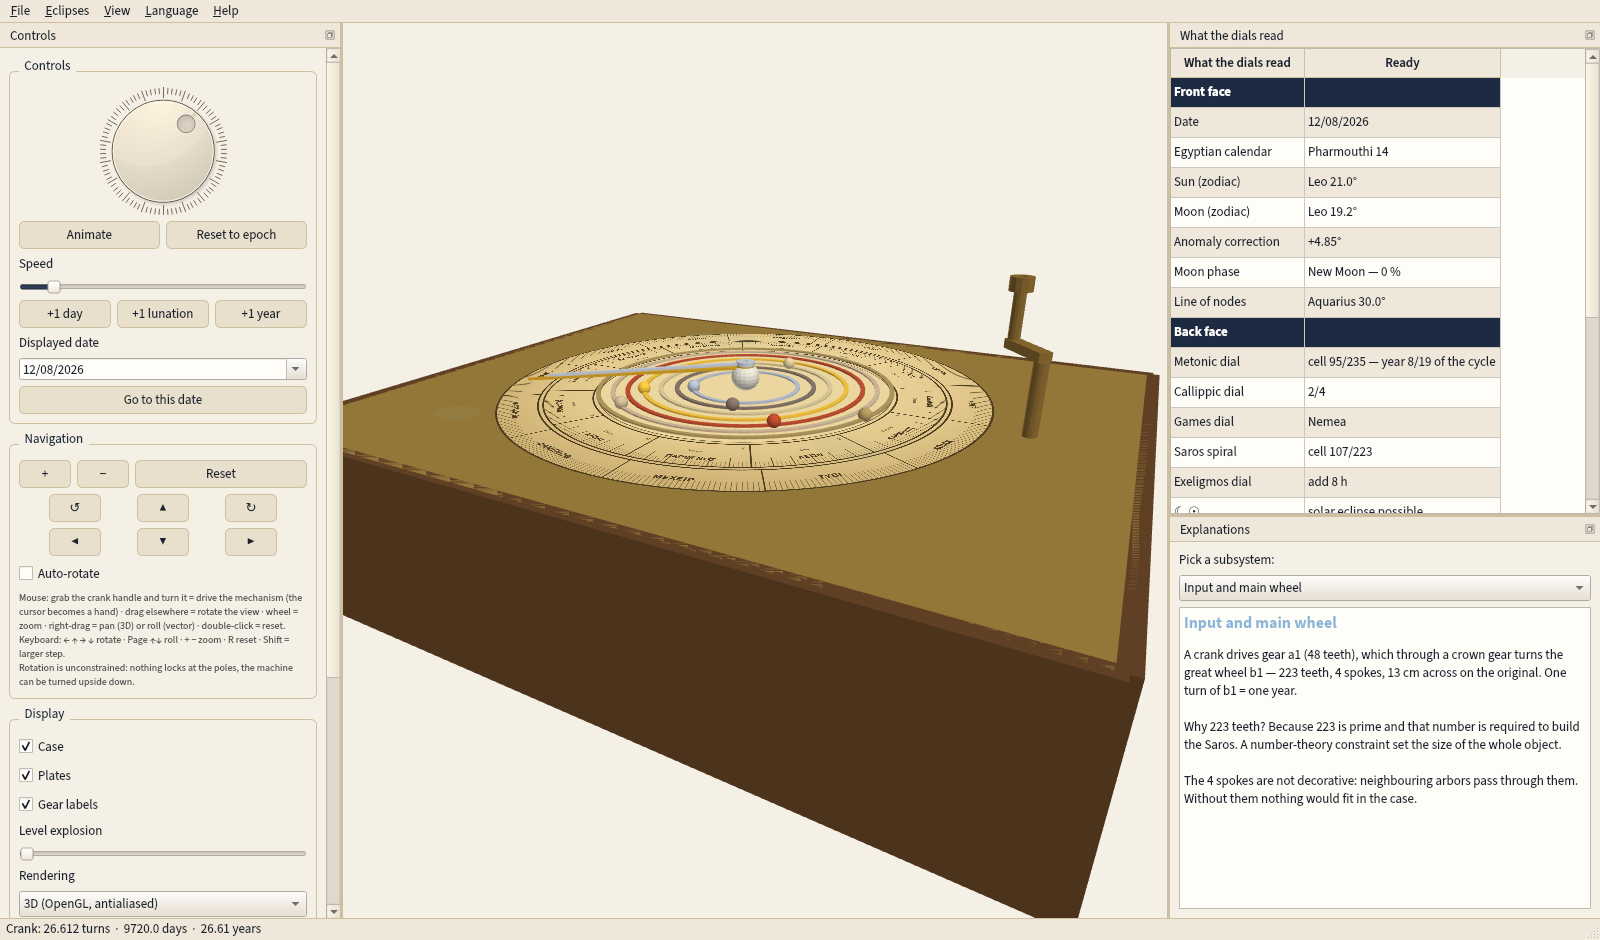
\includegraphics[width=0.86\textwidth]{fenetre-en.png}}\par
\vspace{6mm}
\begin{tcolorbox}[enhanced,width=0.86\linewidth,colback=bronzel,colframe=bronze,arc=4pt,boxrule=1.1pt,left=5mm,right=5mm,top=2.5mm,bottom=2.5mm]
\sffamily\centering
The earliest known astronomical calculator, in working order:\\
\textbf{33 gears} \textbullet{} \textbf{15 arbors} \textbullet{} \textbf{2,231 teeth},
a single crank.
\end{tcolorbox}
\vfill
{\footnotesize\color{summit}\sffamily Exact ratios after Freeth \textit{et al.}, \textit{Nature} 2006 \&
2008, \textit{Scientific Reports} 2021\\[1mm]
Windows \textbullet{} macOS \textbullet{} Linux\par}
\end{titlepage}

\tableofcontents
\newpage

% =====================================================================
\section{Installing the program}

\subsection{The ready-made package}

Packages are on the repository's \textbf{Releases} page
(\fichier{github.com/ARP273-ROSE/Anticythere3D/releases}). Each one \textbf{carries its own
Python}: nothing else to install, and no administrator password is asked for.

\begin{center}
\small
\renewcommand{\arraystretch}{1.25}
\begin{tabularx}{\textwidth}{@{}p{2.5cm}p{6.1cm}X@{}}
\toprule
\rowcolor{lightblue}\textbf{System} & \textbf{File} & \textbf{Installation} \\
\midrule
\textbf{Windows} & \fichier{Anticythere3D-Setup.exe} & run the installer; it installs into
your profile (\fichier{\%LOCALAPPDATA\%\textbackslash Programs}), without administrator
rights \\
\textbf{macOS} Apple Silicon / Intel & \fichier{Anticythere3D-macos-arm64.dmg}\newline
\fichier{Anticythere3D-macos-x86\_64.dmg} & open the disk image, drag the application into
\menu{Applications} \\
\textbf{Linux} x86\_64 / ARM64 & \fichier{Anticythere3D-linux-x86\_64.tar.gz}\newline
\fichier{Anticythere3D-linux-arm64.tar.gz} & unpack, run \fichier{./installer.sh}: installs
into \fichier{\textasciitilde/.local/share}, adds a menu entry, \textbf{no sudo} \\
\bottomrule
\end{tabularx}
\end{center}

These names without a version number are permanent links to the latest release; the
Releases page also lists the same files with their version number, and a
\fichier{SHA256SUMS} file giving the fingerprint of each one.

\begin{attention}[Unsigned packages]
\textbf{Windows}: “Windows protected your PC” — click \menu{More info}, then \menu{Run anyway},
once. \textbf{macOS}: the first time, \textbf{right-click} the application → \menu{Open}, then
confirm; if macOS still refuses: \menu{System Settings → Privacy \& Security → Open Anyway}.
\end{attention}

\subsection{Updates install themselves}

On all three systems, a few seconds after opening, the installed program checks whether a
newer release has been published. If so it offers it, with the release notes in the
interface language; you can also ask with \menu{Help → Check for updates…}. Only a
\textbf{small code archive} is downloaded; its size and fingerprint are checked, it is
unpacked in place of the old one, and the program restarts. When run from source, it
replaces nothing: it offers the download page (or \fichier{git pull}).

\begin{info}[If the update fails]
The message “an application file is in use by another program” means another copy of the
program is running. Close it (or restart the computer) and ask for the update again: the
installed version is left untouched.
\end{info}

\subsection{Incident reports}

If it crashes, freezes or fails to start, the program can tell its maintainer by itself.
\textbf{Nothing is sent without your consent}: the question is asked at first launch, and the
\menu{Help → Send crash reports automatically} option lets you change your mind.
\menu{Help → Report a problem…} sends a written report, in your own words. A report holds
the version, the system and the error trace; no files, no names, no personal paths. Without
a network, it waits for the next start.

\subsection{Where your data lives}

Settings, reports and log are \textbf{never} stored in the program folder, since an update
replaces it entirely:

\begin{center}
\begin{tabularx}{0.92\textwidth}{@{}lX@{}}
\toprule
\rowcolor{lightblue}\textbf{System} & \textbf{Data folder} \\
\midrule
Windows & \fichier{\%LOCALAPPDATA\%\textbackslash Anticythere3D} \\
macOS & \fichier{\textasciitilde/Library/Application Support/Anticythere3D} \\
Linux & \fichier{\textasciitilde/.local/share/Anticythere3D} (or \fichier{\$XDG\_DATA\_HOME}) \\
\bottomrule
\end{tabularx}
\end{center}

\subsection{From source}

All you need is \textbf{Python 3.10 or newer} (on Windows, double-clicking
\fichier{launch.bat} does everything). Everything else — 3D included — is installed by the
program itself on first start: \fichier{python run.py}.

\begin{astuce}[What it installs, and where]
Four packages: \fichier{PyQt6} (the interface), \fichier{numpy} (the geometry),
\fichier{pyqtgraph} and \fichier{PyOpenGL} (the 3D view). Outside a virtual environment it
installs with \fichier{-{}-user}: \textbf{nothing is written into the system's packages}. On
Linux, if Qt lacks system libraries, the program prints the exact command to run.
\end{astuce}

\begin{center}
\begin{tabularx}{0.95\textwidth}{@{}lX@{}}
\toprule
\rowcolor{lightblue}\textbf{Command} & \textbf{Effect} \\
\midrule
\fichier{python run.py -{}-check} & checks dependencies, style, logo and manuals, then exits \\
\fichier{python run.py -{}-no-install} & starts without installing anything \\
\fichier{python run.py -{}-lang fr} & French interface (default: the system's language) \\
\fichier{python run.py -{}-vector} & starts in vector rendering \\
\fichier{python run.py -{}-samples 16} & stronger antialiasing (default: 8) \\
\bottomrule
\end{tabularx}
\end{center}

\begin{attention}[If the 3D view does not start]
On a machine without an OpenGL driver (server, virtual machine, remote desktop),
\textbf{the program does not crash}: it switches by itself to \emph{vector rendering}, which
shows the same motions with no graphics dependency — and exports to SVG and PDF.
\end{attention}

% =====================================================================
\section{Getting started in two minutes}

\begin{enumerate}
  \item Open the program. The machine appears \textbf{closed}, as you would find it on a
        shelf: wooden case, engraved bronze front, hands, crank on the side. The program
        speaks the system's language; the \menu{Language} menu lets you pick English or
        French, and the choice is remembered.
  \item On first launch, one question: allow automatic incident reports or not (see above).
  \item Drive the machine: \textbf{grab the crank handle} with the mouse, on the side, and
        turn it (the cursor becomes a hand) — or turn the \textbf{round knob} at the top left,
        one full turn of which is one year.
  \item Untick \menu{Case}: the case disappears and the 33 gears show up, turning.
  \item Look at the right-hand panel: it permanently shows what the machine's owner read.
\end{enumerate}

\capture{ouvert-en.png}{The case removed, on 12 August 2026: the 33 gears, the 15 arbors and
the two large spoked wheels ($b_1$ at the front, $e_3$ at the back). On the right, the Moon
is new and the panel announces a possible solar eclipse — the one of that very day.}

\begin{astuce}[A look that does not change from one computer to another]
The program imposes its own style (parchment and night-blue colours, the Source Sans 3 font
shipped with it): it looks the same on Windows, macOS and Linux, whether the system uses a
light or a dark theme. Only the screen scaling (125\%, 150\%…) remains the system's.
\end{astuce}

% =====================================================================
\section{The interface}

\subsection{Controls}

\begin{center}
\begin{tabularx}{\textwidth}{@{}lX@{}}
\toprule
\rowcolor{lightblue}\textbf{Item} & \textbf{Role} \\
\midrule
Crank handle & in the view: the machine's \textbf{only} input, grabbed with the mouse (see
below) \\
Round knob & the same crank, geared down: one turn = one year \\
Animate / Pause & turns the crank continuously \\
Speed & simulated days per second \\
+1 day / +1 lunation / +1 year & advances by an exact step \\
Reset to epoch & brings the machine back to its calibration date \\
Displayed date + Go to this date & jumps straight to a date \\
\bottomrule
\end{tabularx}
\end{center}

\begin{info}[Why a single input?]
Because the real machine has only one. Everything else — Sun, Moon, phase, eclipses,
calendars — is not “computed” separately: they are gear ratios, hence mechanical
consequences of the crank's single motion. That is exactly what the program does: no display
formula, only fractions of tooth counts.
\end{info}

\subsection{Turning the crank with the mouse}

\capture{manivelle-en.png}{Before and after one turn of the handle: the date moves from 12/08
to 30/10/2026 (78.6 days), the Moon from new to waning gibbous.}

\begin{enumerate}
  \item Move the mouse onto the crank's \textbf{handle} (or its arm), on the right-hand side
        of the case: the cursor becomes an \textbf{open hand}.
  \item Press and hold the button: the hand closes, the handle is grabbed.
  \item Move in a circle around the crank's axis: the machine moves forwards one way,
        backwards the other. Every dial follows, and so does the round knob.
\end{enumerate}

\begin{info}[How much is one turn of the handle?]
The crank carries wheel $a_1$ (48 teeth), which meshes with the great wheel $b_1$ (223
teeth). One turn of the handle therefore turns $b_1$ by $48/223$ of a turn — and $b_1$ turns
once a year:
\[
  1~\text{turn of the handle} = \frac{48}{223}~\text{year}
  \approx \frac{48}{223}\times 365.24 \approx 78.6~\text{days},
\]
in the opposite direction to $b_1$, as with any two meshing wheels. It takes
$223/48 \approx 4.65$ turns of the handle for one year.
\end{info}

The gesture is the same in \textbf{vector rendering}, where the crank is drawn on wheel
$a_1$. Away from the handle, dragging always rotates the view: you never move the machine by
accident. The mouse wheel turned \emph{over the round knob} also drives the machine.

\subsection{Navigation: zoom, rotate, turn over}

\begin{center}
\begin{tabularx}{\textwidth}{@{}p{5.2cm}X@{}}
\toprule
\rowcolor{lightblue}\textbf{Gesture} & \textbf{Effect} \\
\midrule
Drag the handle & turn the crank (hand cursor) \\
Drag elsewhere & rotate the object \\
Mouse wheel & zoom in forwards, out backwards (bounded: you never go through the machine) \\
Right-drag & pan (3D) or roll (vector) \\
Double-click & reset the view \\
\touche{←} \touche{↑} \touche{→} \touche{↓} & rotate with the keyboard \\
\touche{Page ↑} / \touche{Page ↓} & roll (third axis) \\
\touche{+} / \touche{−} & zoom in / out \\
\touche{R} & reset the view \\
\touche{Shift} held & larger rotation step \\
\touche{Space} & animate / pause \\
\touche{F} / \touche{B} / \touche{I} & front face / back face / three-quarter view \\
\touche{E} & list of upcoming eclipses \\
\touche{F1} & this manual \\
\bottomrule
\end{tabularx}
\end{center}

\begin{astuce}[Truly free rotation]
The camera is driven by a \emph{quaternion}, not by Euler angles: \textbf{nothing locks at the
poles}. You can go over the top, carry on, and turn the machine completely upside down.
\menu{Reset} (or \touche{R}) always brings back exactly the same three-quarter view, whatever
rolls came before.
\end{astuce}

\subsection{Display}

\begin{center}
\begin{tabularx}{\textwidth}{@{}lX@{}}
\toprule
\rowcolor{lightblue}\textbf{Setting} & \textbf{Effect} \\
\midrule
\textbf{Case} & shows or removes the case and the front (the crank stays, so it can be
grabbed) \\
Plates & the two inner plates that carry the arbors \\
Gear labels & labels each gear with its tooth count \\
Level explosion & spreads the 16 meshing planes apart along the arbors \\
\textbf{Rendering} & real-time 3D, or exportable vector \\
\textbf{Tooth profile} & triangular (ancient) or involute (modern) \\
Highlight & lights up one subsystem only, fades the others \\
\bottomrule
\end{tabularx}
\end{center}

\begin{info}[The two tooth profiles]
The teeth of the real machine are \textbf{nearly equilateral triangles}. The \emph{mean} ratio
is then strictly exact — which is why the instrument is right — but the \emph{instantaneous}
ratio wobbles as each tooth passes. The \textbf{involute of a circle}, unknown to the Greeks,
is the only profile giving a constant ratio at every instant.
\end{info}

\subsection{Level explosion}

\capture{eclatement-en.png}{Explosion at 0, 50 and 100\%: the stack stretches along the
arbors, no gear leaves its plane.}

The 33 gears are arranged on \textbf{16 levels}: two gears on the same level lie in the same
plane and mesh. The \menu{Level explosion} slider widens the gap between two levels from
3.4~mm (assembled machine) to 15.4~mm:
\begin{itemize}
  \item the \textbf{back} stays in place and the stack stretches forwards; the front (dials,
        Cosmos, hands, crank) moves with the first level;
  \item \textbf{no gear moves within its plane}; meshing gears stay face to face, and the
        order of the levels never changes;
  \item the \textbf{arbors lengthen} with the stack: no gear floats;
  \item in vector rendering the slider is greyed out: the explosion would happen along the
        line of sight.
\end{itemize}

\begin{info}[No part goes through another]
The test suite checks, at six slider positions and for 76 angles of the carrier $e_3$, that
no gear enters another and that no arbor, \textbf{extended to its dial}, passes through a gear.
This check led to two fixes in version 1.3.1: arbor $o$ of the Callippic hand went through
wheel $i_1$ of the Exeligmos (it was moved along its pitch circle around $p$, keeping the
exact centre distance); wheels $k_1$, $k_2$ of the pin and slot, which turn with $e_3$, swept
through arbors $b$ and $l$ (they now sit just in front of $e_3$, which carries them).
\end{info}

\capture[0.55]{arbre_o_callippique.png}{The Callippic train highlighted (exploded machine,
three-quarter back view): arbor $o$ runs down to its dial without going through any gear.}

\subsection{The colours of the seven trains}

Each subsystem has its colour, in the 3D view, in the vector rendering and its exports, and in
the legend. \menu{Highlight} lights up just one:

\capture[0.62]{evidence-saros-en.png}{The Saros train highlighted, the others faded.}

\begin{center}
\small
\begin{tabularx}{\textwidth}{@{}lllX@{}}
\toprule
\rowcolor{lightblue}\textbf{Colour} & \textbf{Code} & \textbf{Train} & \textbf{Gears} \\
\midrule
\pastille{trinput} orange & \fichier{\#DE6910} & Input and main wheel & $a_1$, $b_1$, $b_2$ \\
\pastille{trmoon} blue & \fichier{\#0D59C1} & Moon train & $b_3$, $c_1$, $c_2$, $d_1$, $d_2$, $e_1$, $e_2$, $e_5$, $e_6$ \\
\pastille{tranomaly} blood red & \fichier{\#8E1700} & Lunar anomaly (pin and slot) & $e_3$, $e_4$, $k_1$, $k_2$ \\
\pastille{trmetonic} teal & \fichier{\#1D9594} & Metonic cycle & $l_1$, $l_2$, $m_1$, $m_2$, $n_1$ \\
\pastille{trcallippic} khaki & \fichier{\#786F4C} & Callippic cycle & $n_2$, $p_1$, $p_2$, $o_1$ \\
\pastille{trsaros} raspberry & \fichier{\#841959} & Saros (eclipses) & $m_3$, $f_1$, $f_2$, $g_1$ \\
\pastille{trexeligmos} lilac & \fichier{\#B66CCD} & Exeligmos & $g_2$, $h_1$, $h_2$, $i_1$ \\
\bottomrule
\end{tabularx}
\end{center}

\begin{info}[A computed palette, not picked by eye]
The seven hues come out of an optimisation (\fichier{anticythere/palette.py}): a CIEDE2000
colour difference of at least 27.7 between all of them with normal vision; under simulated
deuteranopia and protanopia, at least 19 between touching trains and 12 between all; a
contrast of at least 3:1 on the parchment background. The tests check these thresholds at
every release.
\end{info}

\subsection{Vector rendering and exports}

\capture{vectoriel-en.png}{Vector rendering of the front face, with its legend: every tooth is a
curve, not a pixel.}

This mode draws the \textbf{real tooth outlines} as curves. It serves three purposes:
\begin{itemize}
  \item looking at the mechanism flat, with nothing hidden;
  \item exporting to \textbf{SVG} or \textbf{A3 PDF} (\menu{File}) — the files contain no
        bitmap image: print at A0 or zoom forever;
  \item working on a machine without OpenGL.
\end{itemize}

The \menu{File} menu also offers a PNG screenshot of the window, a CSV export of the dial
panel, and an \textbf{STL} export of the 33 gears, ready for 3D printing (0.15~mm clearance and
3.2~mm bore already applied, with a bill of materials).

\capture[0.8]{enregistrer-en.png}{The save dialog: a real file explorer, with its shortcuts (home
folder, Desktop, Documents, Pictures, Downloads), the folder tree, folder creation and the file
type filter.}

\begin{astuce}[On Linux too, a real file explorer]
On Linux, the “native” dialog often goes through a portal that reduces it to a plain list.
The program therefore imposes Qt's full dialog there, shown above, with the usual places in
the side bar and mounted media (USB sticks, disks). On Windows and macOS it uses the system's
dialog, which is already complete.
\end{astuce}

% =====================================================================
\section{What the dials show}

\subsection{The readings panel}

The right-hand panel can be detached (it is a window in its own right) and shows:

\begin{center}
\small
\begin{tabularx}{\textwidth}{@{}lX@{}}
\toprule
\rowcolor{lightblue}\textbf{Row} & \textbf{Meaning} \\
\midrule
Date & Gregorian date matching the crank's position \\
Egyptian calendar & month and day of the 365-day calendar on the front \\
Sun (zodiac) & position of the mean Sun — also the date pointer \\
Moon (zodiac) & position of the Moon, anomaly included \\
Anomaly correction & offset produced by the pin and slot, at most $\pm 6.58°$ \\
Moon phase & name of the phase and illuminated percentage \\
Line of nodes & position of the nodes, which decides eclipses \\
Metonic dial & cell out of 235 and year out of 19 of the cycle \\
Callippic dial & quarter out of 4 of the 76-year cycle \\
Games dial & panhellenic games of the year \\
Saros spiral & cell out of 223 \\
Exeligmos dial & time correction to add: 0, 8 or 16 hours \\
\textbf{Moon and Sun} & possible or near-certain eclipse warning \\
Planets (2021 model) & positions after the model of Freeth \textit{et al.} (2021) \\
Mechanism vs real sky & \textbf{the instrument's own error}, in degrees \\
\bottomrule
\end{tabularx}
\end{center}

\begin{info}[The last row is the most interesting one]
The program constantly compares what the machine shows with modern ephemerides. For the mean
Sun the difference is \textbf{zero}: the ratio is exactly 1. For the Moon it reaches a few
degrees per century, and that is not a software fault — it is the instrument's real error:
\[
\underbrace{2.2°}_{\substack{\text{evection and variation}\\ \text{not mechanised}}}
\;+\;
\underbrace{3.5°\ \text{per 50 years}}_{\substack{\text{drift of}\\ 254/19}}
\;+\;
\underbrace{0.8°}_{\substack{\text{precession of}\\ \text{the apogee}}}
\]
The test suite checks that the measured error stays within this budget: the simulator is
faithful \emph{down to its flaws}.
\end{info}

\subsection{Eclipses}

\menu{Eclipses → Upcoming eclipses…} (key \touche{E}) lists the next twelve eclipses from the
displayed date; a double-click, or \menu{Go to this date}, takes the machine there.

\capture[0.78]{eclipses-en.png}{From 12 August 2026: the total solar eclipse of that very day
(distance to node 14.35°), then the lunar eclipse of 28 August.}

\begin{info}[What the “Distance to node” column says]
An eclipse is only possible at a new or full Moon close to a node of the lunar orbit. Below
15.4°, a solar eclipse is central somewhere on Earth; beyond 18.5° there is none. The dates in
the list come from modern ephemerides, to within a few minutes: they are a reference for
judging the machine, which itself only knows the Saros cell.
\end{info}

\subsection{Reading the inscriptions}

The dials carry inscriptions, reproduced from the fragments. Turn the machine over (key
\touche{B}) and zoom in: everything is engraved as vectors, sharp at any magnification.

\capture[0.62]{vectoriel-arriere-en.png}{The back face in vector rendering, mechanism showing
through: Metonic spiral at the top, Saros spiral at the bottom, the great four-spoked wheel
$e_3$ that carries the pin and slot.}

\begin{center}
\small
\begin{tabularx}{\textwidth}{@{}llX@{}}
\toprule
\rowcolor{lightblue}\textbf{Dial} & \textbf{Divisions} & \textbf{What is written} \\
\midrule
\multicolumn{3}{@{}l}{\textit{Front face}}\\
Zodiac & $12 \times 30°$ & the twelve signs in Greek from the vernal point; note
\emph{Ch\^elai}, “the claws”, where we say Libra \\
Parapegma & letters & small index letters scattered in the zodiac, pointing to a star
calendar engraved on the plate \\
Calendar & 365 days & the Egyptian months in Greek letters; the ring is \textbf{movable}, shifted
one notch every four years \\
\midrule
\multicolumn{3}{@{}l}{\textit{Back face}}\\
Metonic & spiral, 235 cells & one cell = one lunar month, with the name of its Corinthian month;
the year number in Greek numerals marks each of the 19 years \\
Callippic & 4 sectors & which of the four 76-year cycles is running \\
Games & 4 sectors & \emph{Olympia}, \emph{Nemea}, \emph{Isthmia}, \emph{Pythia} — the only
non-astronomical dial \\
Saros & spiral, 223 cells & the cells where an eclipse is possible carry $\mathrm{H}$ (eta, for
\emph{H\^elios}, the Sun) or $\Sigma$ (sigma, for \emph{Sel\^en\^e}, the Moon) \\
Exeligmos & 3 sectors & 0, 8 or 16 hours to \textbf{add} to the time read on the Saros \\
\bottomrule
\end{tabularx}
\end{center}

\begin{info}[The seven thirteen-month years]
Nineteen solar years make 235 lunar months, but $19 \times 12 = 228$: seven years of the cycle
have \textbf{thirteen} months. They are spread by the criterion $(12k) \bmod 19 < 7$, i.e.\
years $2, 5, 8, 10, 13, 16, 19$ — and the total comes back to exactly 235 cells. That is why
the year-start marks are not evenly spaced on the spiral.
\end{info}

\begin{info}[Why 223 cells on the Saros]
Three lunar periods coincide there to within five hours over eighteen years: 223 synodic
months (same phase), 242 draconic (same node), 239 anomalistic (same distance). The eclipse
repeats. A remainder of $0.321$ day shifts it by $7.7$~hours — about $116°$ of longitude.
After three Saros, that remainder is almost a whole day: this is what the Exeligmos dial
counts.

\textbf{Caveat}: the eclipse glyphs are \textbf{computed}, not copied. The plate's pattern is
known only from fragments; the program applies the criterion the machine mechanises — syzygy
close to a node — over the 223 months of a Saros, and marks 48 solar cells and 32 lunar ones,
22 of which carry both.
\end{info}

% =====================================================================
\section{The ratios, and why they are exact}

\menu{Help → The mathematics of the mechanism} gives the full table. Ratios are kept as
\textbf{exact fractions}, never as decimal numbers:

\begin{center}
\begin{tabularx}{\textwidth}{@{}llX@{}}
\toprule
\rowcolor{lightblue}\textbf{Output} & \textbf{Ratio} & \textbf{Check} \\
\midrule
Sidereal Moon & $254/19$ & sidereal month of 27.321\,266 d \\
Carrier $e_3$ & $477/4237$ & 8.8826 years (real apogee: 8.8504) \\
Anomaly & — & period of \textbf{27.5533 d} against 27.554\,55: \textbf{1.8 minutes} \\
Metonic & $5/19$ & 5 turns in 19 years \\
Callippic & $1/76$ & 1 turn in 76 years \\
Saros & $940/4237$ & 4 turns for 223 lunations \\
Exeligmos & $235/12711$ & 1 turn in 54.09 years, i.e. 3 Saros \\
\bottomrule
\end{tabularx}
\end{center}

\begin{info}[The anomalistic month is written nowhere]
The pin and slot are mounted on wheel $e_3$, which turns in 8.88 years — the precession of the
lunar apogee. The modulation's period is therefore the \emph{difference} between the two
rotations:
\[
  \frac{254}{19} - \frac{477}{4237} = \frac{56\,165}{4237}\ \text{turn/year}
  \quad\Longrightarrow\quad T = 27.553\ \text{days},
\]
to be compared with the real anomalistic month of 27.554\,55 days: \textbf{1.8 minutes apart}.
This number appears on no wheel: it emerges from a subtraction of frequencies made in bronze.
\end{info}

% =====================================================================
\section{The Help menu}

\begin{center}
\begin{tabularx}{\textwidth}{@{}p{6.2cm}X@{}}
\toprule
\rowcolor{lightblue}\textbf{Entry} & \textbf{Effect} \\
\midrule
Manual (PDF) \hfill\touche{F1} & opens this manual, in the interface language \\
Check for updates… & queries the published releases \\
Report a problem… & sends a written report \\
Send crash reports automatically & consent given or withdrawn \\
Quick guide & built-in summary, with the colour legend \\
The mathematics of the mechanism & table of the exact ratios \\
Keyboard shortcuts & every shortcut and gesture \\
About & version, sources, and the program's logo \\
\bottomrule
\end{tabularx}
\end{center}

\capture[0.5]{a-propos-en.png}{The “About” window: the logo is the same as the icon's, the
installer's and this manual's — one single drawing, the four-spoked great wheel $b_1$ and the
Saros spiral.}

% =====================================================================
\section{Troubleshooting}

\begin{center}
\small
\begin{tabularx}{\textwidth}{@{}p{5.4cm}X@{}}
\toprule
\rowcolor{lightblue}\textbf{Symptom} & \textbf{What to do} \\
\midrule
“Missing dependencies” (source) & run \fichier{python run.py} again, or
\fichier{pip install -r requirements.txt} \\
Black window, no 3D & OpenGL unavailable: switch to \textbf{vector rendering} (the program does
it by itself) \\
Jagged teeth & raise the antialiasing: \fichier{-{}-samples 16}, or use vector rendering \\
Animation too slow & lower the speed, untick \menu{Gear labels} \\
Only the large wheels are visible & expected: $b_1$ and $e_3$ cover the small ones. Use
\menu{Level explosion} or \menu{Highlight} \\
The crank cannot be grabbed & aim at the handle itself: the cursor must become a hand \\
The view is tilted or upside down & \menu{Reset} or \touche{R} \\
“Windows protected your PC” & unsigned installer: \menu{More info} → \menu{Run anyway} \\
macOS refuses to open the application & right-click → \menu{Open}, or System Settings →
Privacy \& Security → Open Anyway \\
The update fails & close the other copy of the program, then ask again \\
\bottomrule
\end{tabularx}
\end{center}

% =====================================================================
\section{What is faithful, and what is not}

\begin{astuce}[Faithful and checked]
The 30 attested gears and their tooth counts, the ratios of every train, the pin-and-slot
device and its carrier, the back dials (Metonic spiral of 5 turns and 235 cells, Saros spiral
of 4 turns and 223 cells), the principle of the single crank, the four spokes of $b_1$.
\end{astuce}

\begin{attention}[Reconstructed or simplified]
\begin{itemize}
  \item The \textbf{planets} are computed after the 2021 model, but not modelled in 3D: they
        are reconstructions, not surveys.
  \item The \textbf{layout of the arbors} is computed by constrained optimisation; it keeps the
        17 exact centre distances, but it is not the original's arrangement, which remains
        partly unknown.
  \item The Saros \textbf{eclipse glyphs} are computed, not copied from the plate, known only
        from fragments.
  \item The \textbf{order of the levels} is the project's, not a survey: $k_1$, $k_2$ are
        carried by $e_3$ as in the reconstructions by Freeth \textit{et al.}, but the stacking
        of the other trains is chosen so that no arbor goes through a gear.
  \item The \textbf{case} follows the proportions of the reconstructed mechanism, not the
        original's 34~$\times$~18~$\times$~9~cm.
\end{itemize}
\end{attention}

\vfill
\begin{tcolorbox}[enhanced,colback=parchemin,colframe=summit,arc=2mm,boxrule=0.6pt]
\small
\textbf{Sources.} Freeth T. \textit{et al.}, \textit{Nature} \textbf{444} (2006) 587–591;
Freeth T., Jones A., Steele J., Bitsakis Y., \textit{Nature} \textbf{454} (2008) 614–617;
Freeth T., Higgon D., Dacanalis A., MacDonald L., Georgakopoulou M., Wojcik A.,
\textit{Scientific Reports} \textbf{11}:5821 (2021); Meeus J., \textit{Astronomical
Algorithms}, 2nd ed.
\end{tcolorbox}

\end{document}
